% Generated from ../chapters/03-emergence-feedback-and-downward-causation.md
\chapter{Chapter 3 --- Emergence, Feedback, and Downward Causation}\label{chapter-3-emergence-feedback-and-downward-causation}

Complex systems are often introduced through \textbf{emergence}: large-scale patterns produced by interactions among smaller components. Water molecules do not individually contain a wave. Birds following local rules can form a flock. Buyers and sellers produce market prices that no participant directly commands. Neurons produce perception through coordinated activity.

Emergence is only half of the story. Once a higher-level pattern exists, it changes the conditions experienced by the parts. This influence is commonly called \textbf{downward causation} or \textbf{top-down causation} \autocite{ellis2012topdown,noble2012biological}. The term does not imply a mysterious force descending from a separate realm. It means that the state of a larger organization constrains lower-level interactions.

A physical example is a crystal. The lattice structure constrains the energy states available to electrons. The lattice is made of atoms, yet once formed it affects how those atoms and electrons behave. In fluid dynamics, the geometry of a container constrains possible flows. In a computer, software is physically implemented by electronics, but the running program determines which circuits switch at a given moment.

A social example is a university. It consists of people, buildings, documents, and machines. Yet the institution constrains individuals through roles, schedules, standards, budgets, and expectations. A professor's actions cannot be predicted from neurons alone; they depend on the lecture, the curriculum, and the meaning of the role. The institutional level is not independent of people, but it is causally relevant.

The human body is a hierarchy of such constraints. A project changes attention and daily behaviour. Behaviour changes sleep, movement, nutrition, and social interaction. These alter autonomic, endocrine, immune, and mechanical signals. Cells respond by changing metabolism, gene expression, proliferation, and matrix production. The high-level purpose is implemented molecularly, but its causal description cannot be replaced by listing molecules.

\begin{figure}
\centering
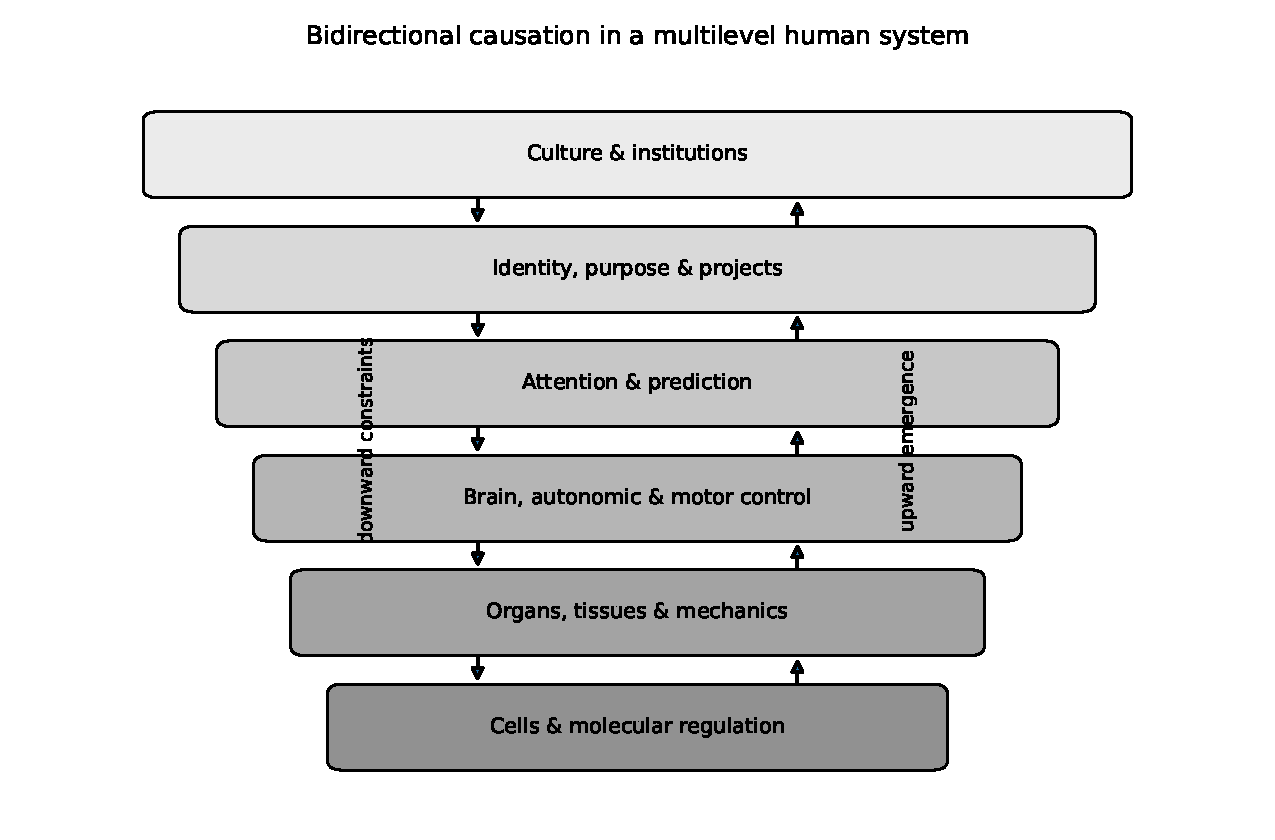
\includegraphics[width=0.82\textwidth]{../figures/causal-hierarchy-v4.pdf}
\caption{Causation in a multilevel system runs both upward and downward. Lower levels make higher levels possible; higher levels constrain the conditions under which lower levels operate.}
\end{figure}

Feedback closes the loop. Better movement changes sensory evidence, which changes prediction and confidence, which makes better movement more likely. Chronic pain can form the opposite loop: anticipated pain increases guarding, guarding redistributes load, load increases irritation, and irritation confirms the expectation.

This is where belief becomes biologically relevant without magical thinking. A belief is not merely a sentence. It is a stable expectation that influences attention and action. ``I am fragile'' changes which movements are attempted and how they are performed. Over years, the resulting loads alter tissues. Culture enters the body through repeated constraints.

Downward causation also clarifies the proposed role of practice. Meditation or Tai Chi does not directly instruct a chromosome to rejuvenate. It changes high-level constraints: attention, threat prediction, voluntary control, breathing, movement, and daily behaviour. Those changes propagate through ordinary physiological pathways. The open empirical question is how deep and how far the cascade can go.

The strongest version of the framework therefore does not oppose bottom-up biology. It proposes \textbf{causal closure across levels}: molecules enable tissues; tissues enable organisms; organisms create contexts that regulate molecules. No single level is always the true cause. The useful level depends on the question.

\section{Downward causation is not downward magic}\label{downward-causation-is-not-downward-magic}

Critics sometimes object that because higher levels are made of lower levels, all causation must ultimately be bottom-up. This confuses implementation with explanation. A traffic law is implemented through human nervous systems, engines, roads, and signals. Yet the law changes traffic because people interpret and enforce it. Removing the legal level would make prediction worse, not more scientific.

Similarly, the statement ``stress changes gene expression'' does not claim that an abstract idea bypasses chemistry. It identifies a causal chain whose higher-level description carries information that a molecular list omits.

\section{Constraint as a mechanism}\label{constraint-as-a-mechanism}

Higher levels often act by restricting possibilities rather than supplying force. A container does not push every fluid molecule into a vortex; its geometry limits possible flows. A social institution does not control every thought; it restricts roles and incentives. A tissue boundary constrains cell migration. A belief constrains which actions are attempted.

This is why the language of \textbf{constraint} is central. Downward causation is frequently the propagation of boundary conditions through a hierarchy.

\section{The body as a society of cells}\label{the-body-as-a-society-of-cells}

Multicellular life can be viewed as an ancient social contract. Cells surrender unlimited reproduction, specialize, exchange resources, and accept coordinated death. Cancer is partly a breakdown of this cooperation. The organism-level pattern constrains each cell, while cells maintain the organism that constrains them.

The analogy with society is imperfect but illuminating. A healthy society cannot be understood by psychology alone, and a healthy body cannot be understood by molecular biology alone. In both cases, institutions or tissues stabilize collective identities that feed back on components.
